\section{Additional Notes}

\subsection{Source code}
The source code is overall well developed and the general structure of the code follows the MVC pattern as stated in the DD.

We also noted that parts of the PHP code doesn't have documentation, while Phyton is well documented.

\subsection{Logic concerns}
During the testing of the application we encountered some bad behaviours.
The example found by us were:
\begin{itemize}
    \item When a Farmer, while inserting two New Production Data, try to completely harvest one of the crop of its plantation in two different times (the second value exceed the remaining area to be harvested), in the "Production Data" the page remains bugged with the crop, that the farmer try to completely harvest, and an area value that we didn't understand how it was produced.
    \begin{figure}[h!]
        \centering
        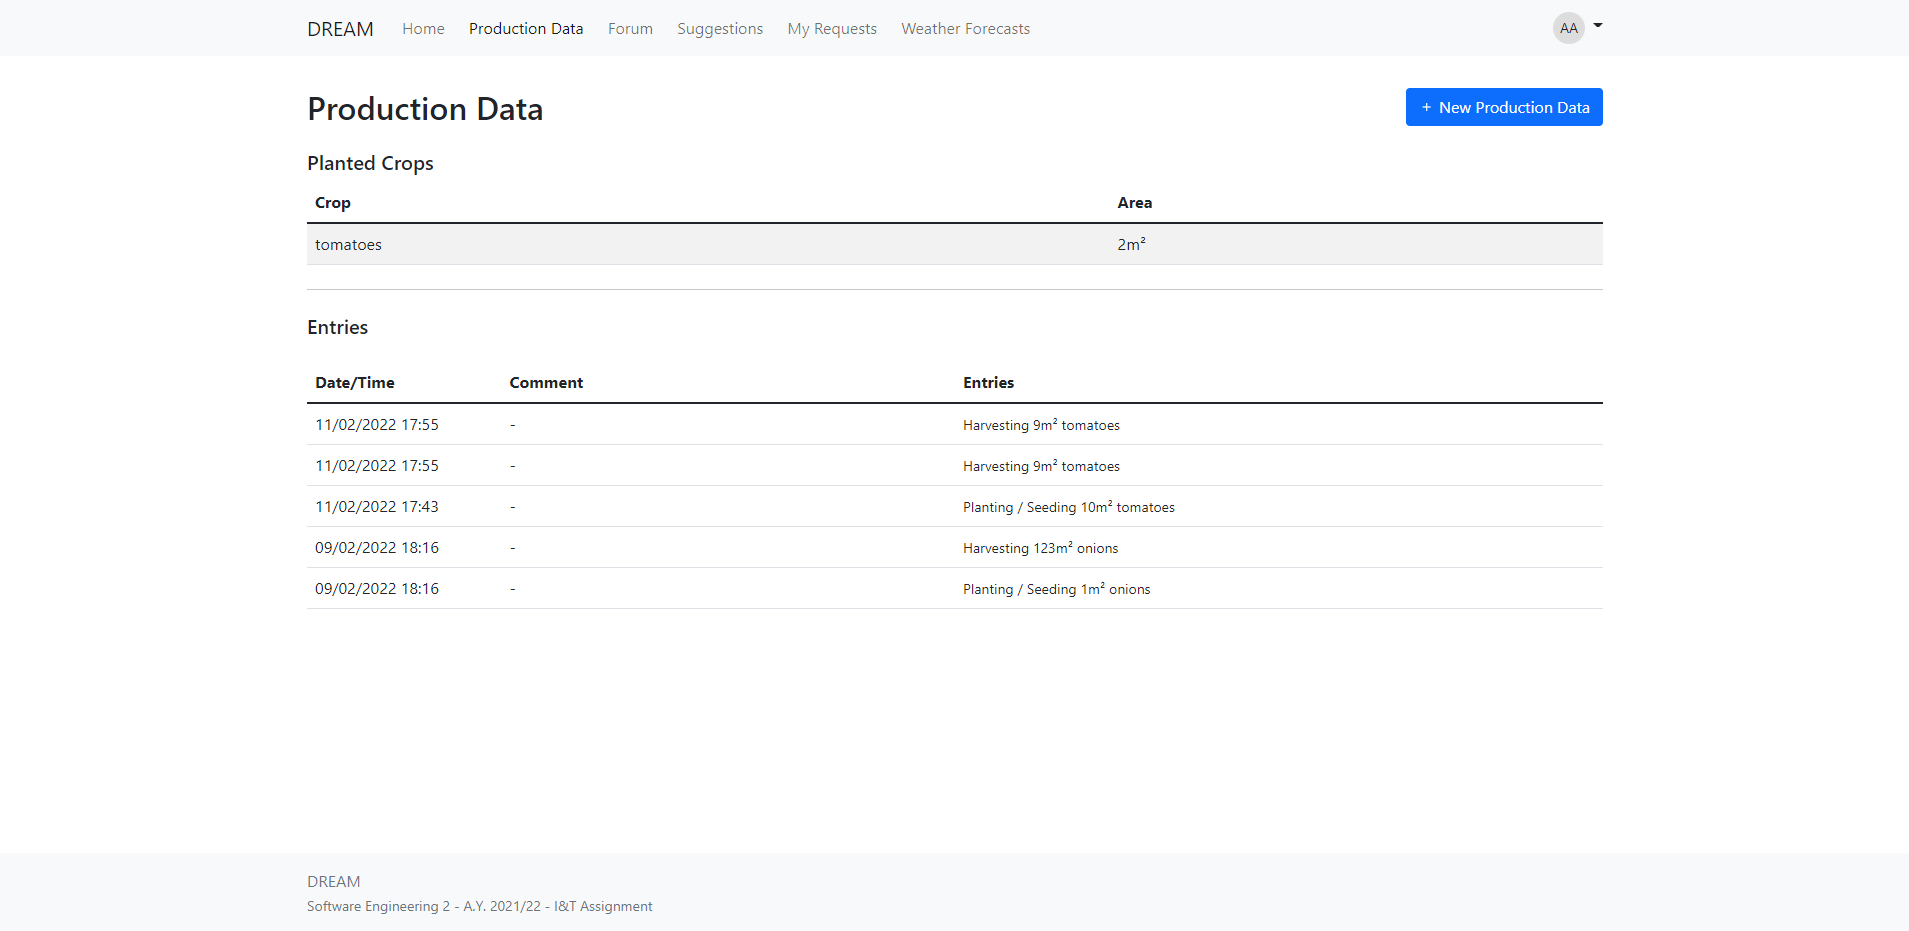
\includegraphics[scale=0.25]{images/additional_notes/fail_inserting_double_production_harvesting.png}
        \caption{Double harvesting in production data}
        \label{fig:double_harvesting_production_data}
    \end{figure}
   \FloatBarrier
    Whenever this bug happens other bad behaviours will occur if the Farmer tries to insert another crop in a New Production Data.
    \begin{figure}[h!]
        \centering
        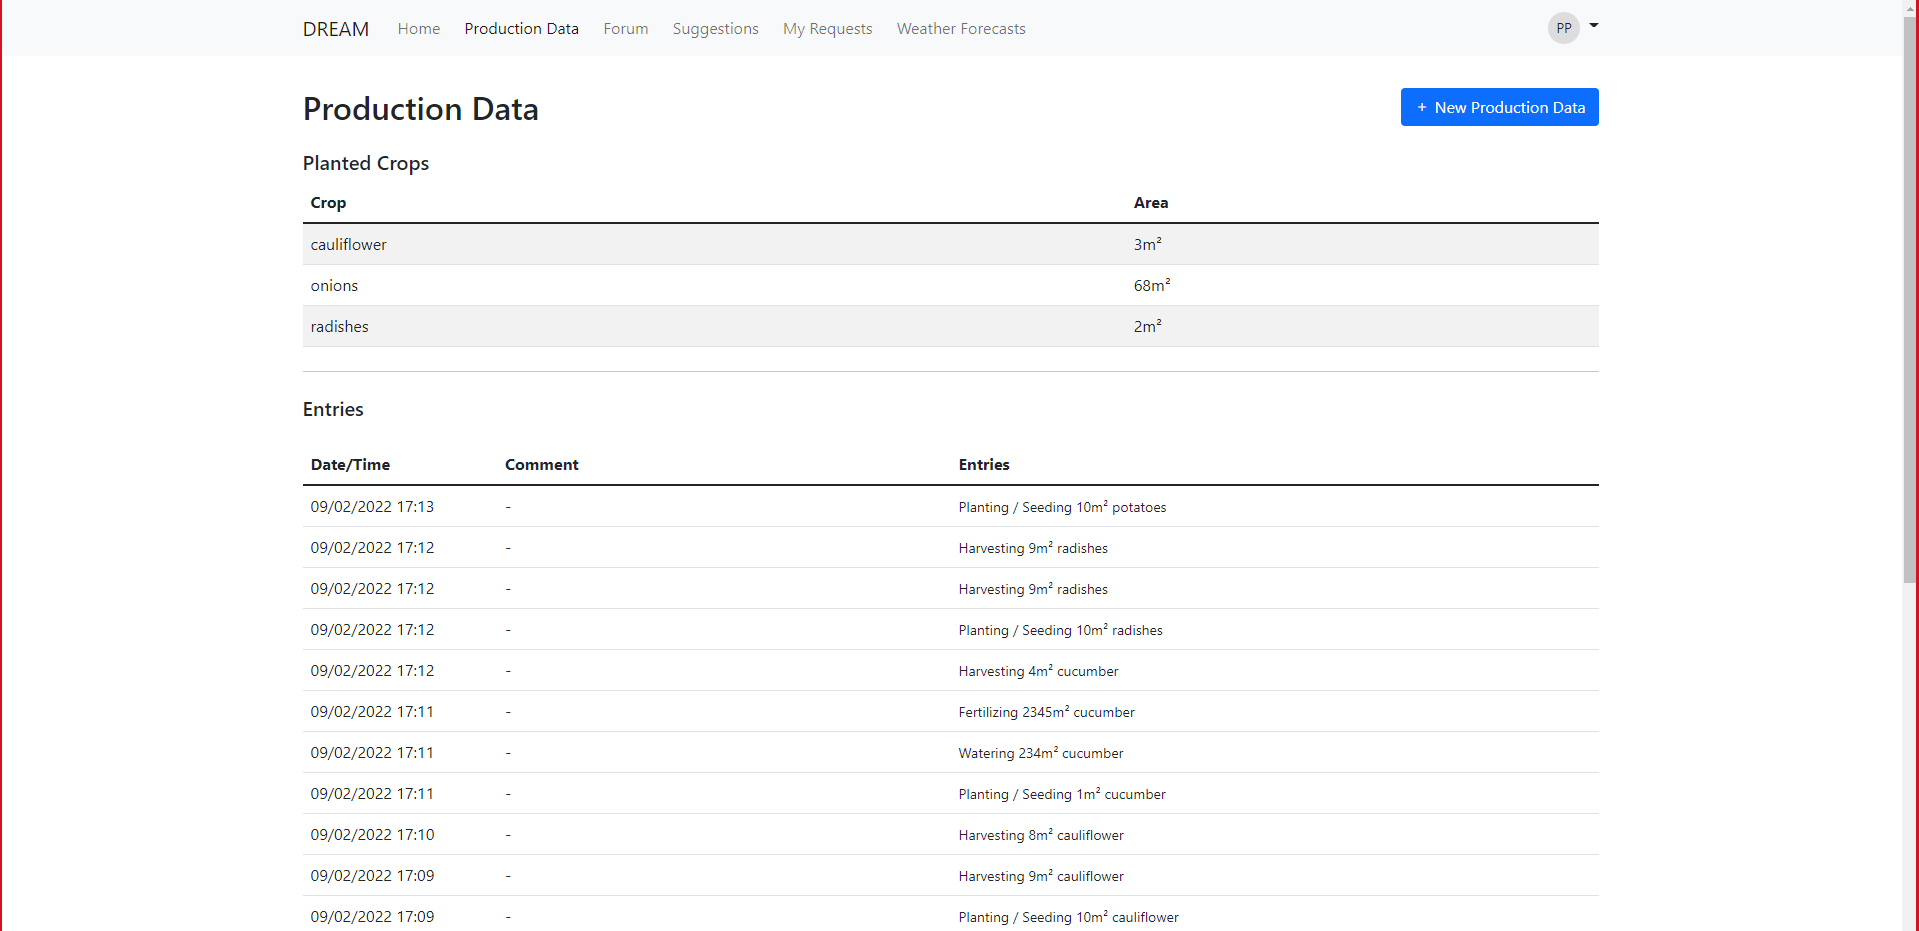
\includegraphics[scale=0.25]{images/additional_notes/insert_something_not_present_in_production_data.png}
        \caption{Crop not inserted from production data}
        \label{fig:fail_insert_data_from_production_data}
    \end{figure}
   \FloatBarrier
    \item When a Farmer tries to insert a New Production Data concerning Fertilizing, Watering or Harvesting, if the User select "Select an entry" instead of selecting a real crop, the system display a server related error.\\
    Screen before the error:
    \begin{figure}[h!]
        \centering
        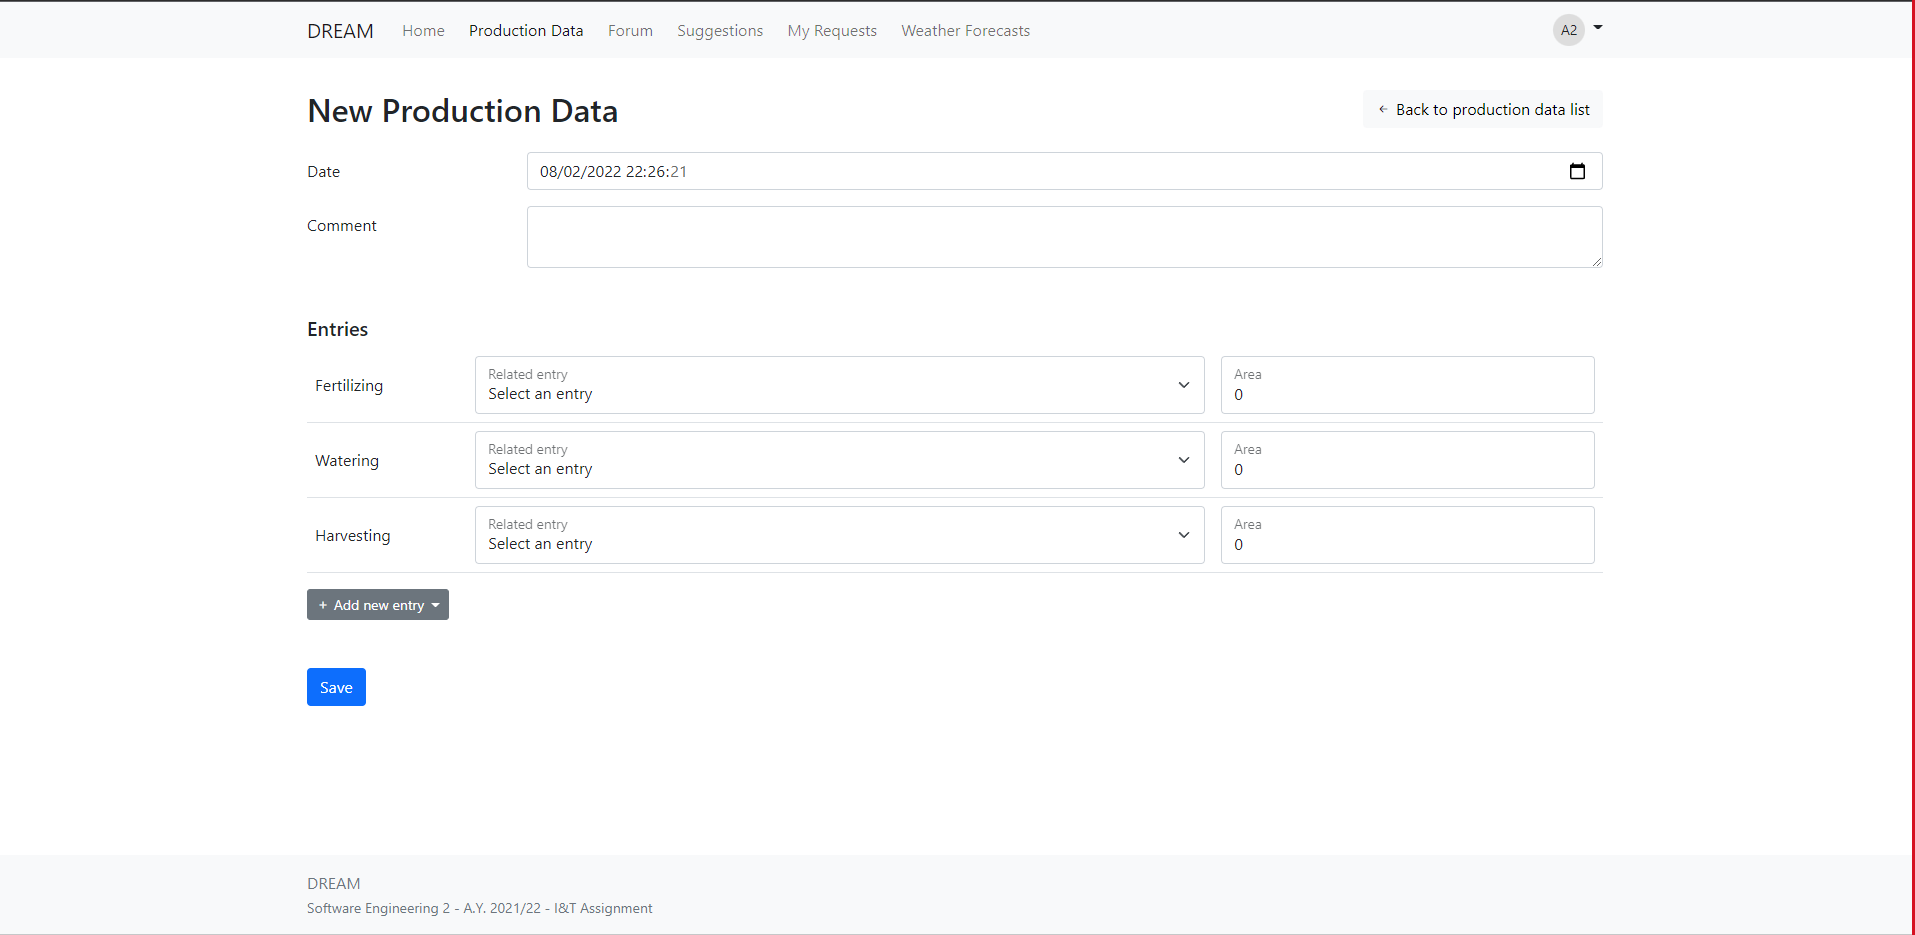
\includegraphics[scale=0.25]{images/additional_notes/production_data_screen.png}
        \caption{Example of selection that retrieves an error}
        \label{fig:my_label}
    \end{figure}
   \newpage
    Error screen:
    \begin{figure}[h!]
        \centering
        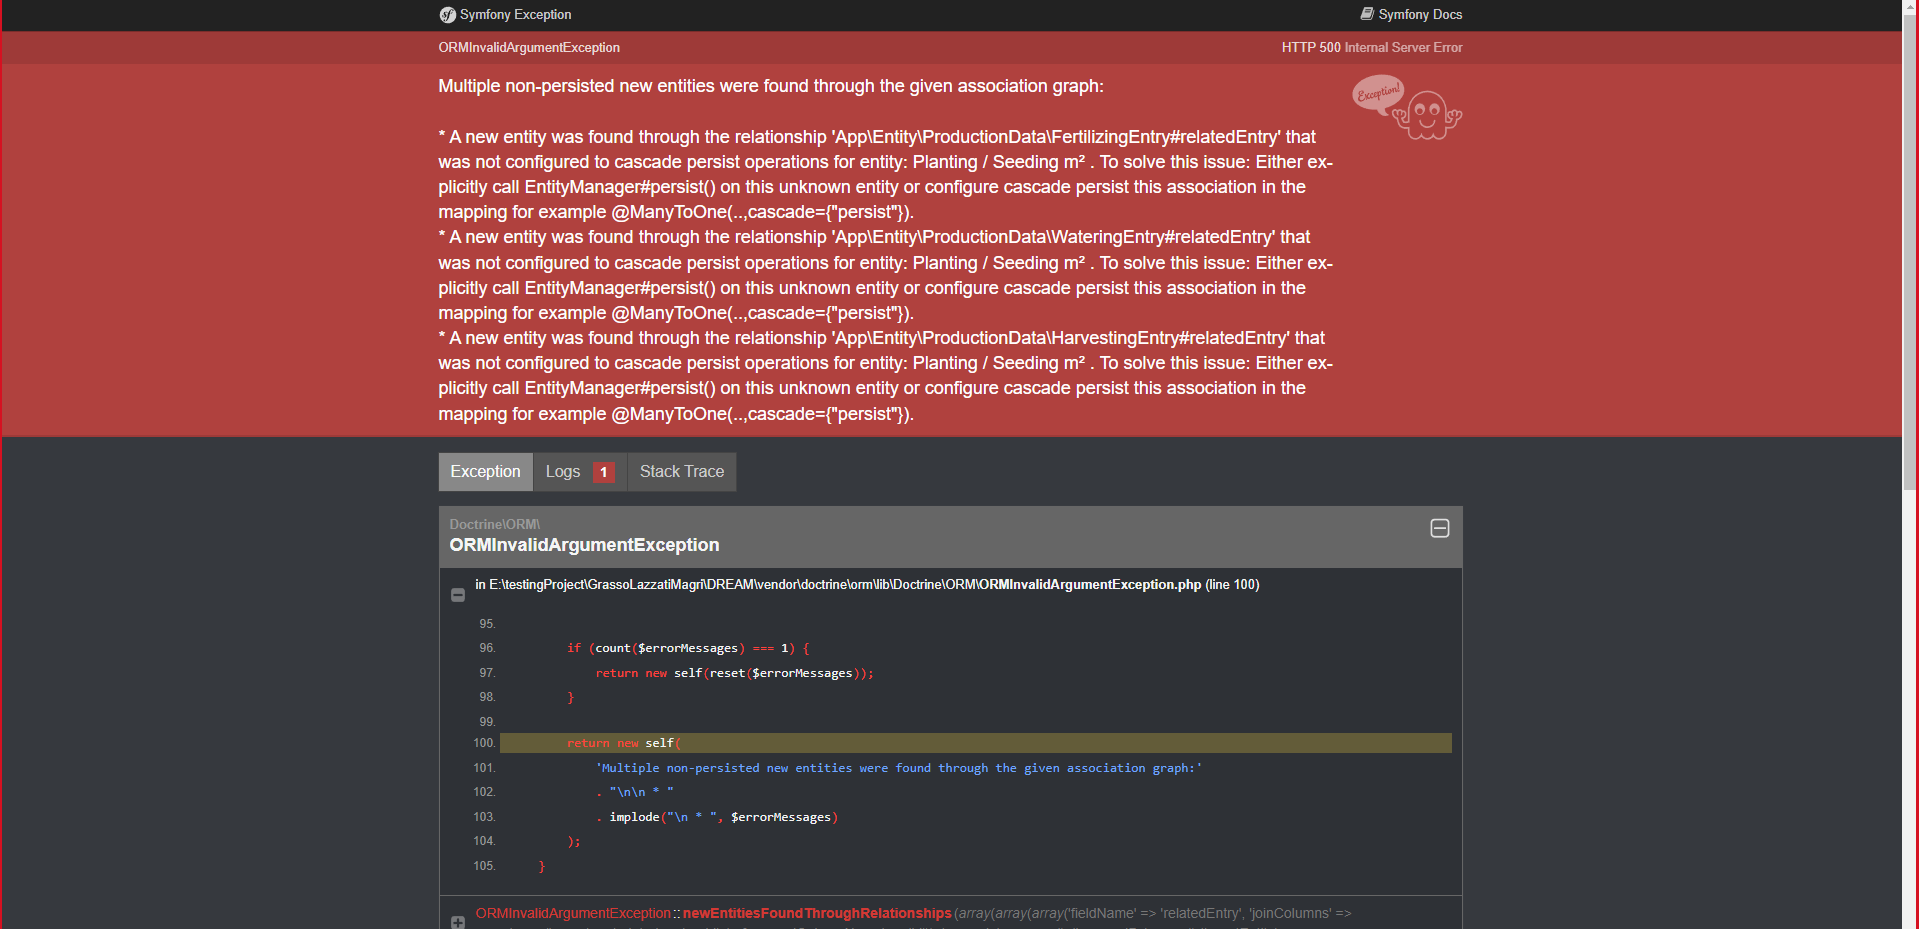
\includegraphics[scale=0.25]{images/additional_notes/production_data_screen_error.png}
        \caption{Error retireved}
        \label{fig:my_label}
    \end{figure}
    \FloatBarrier
    \item When an Agronomist tries to see the details of a farm to visit that he has inserted in the Daily Plan, the system display a server related error.\\
    Screen before the error:
    \begin{figure}[h!]
        \centering
        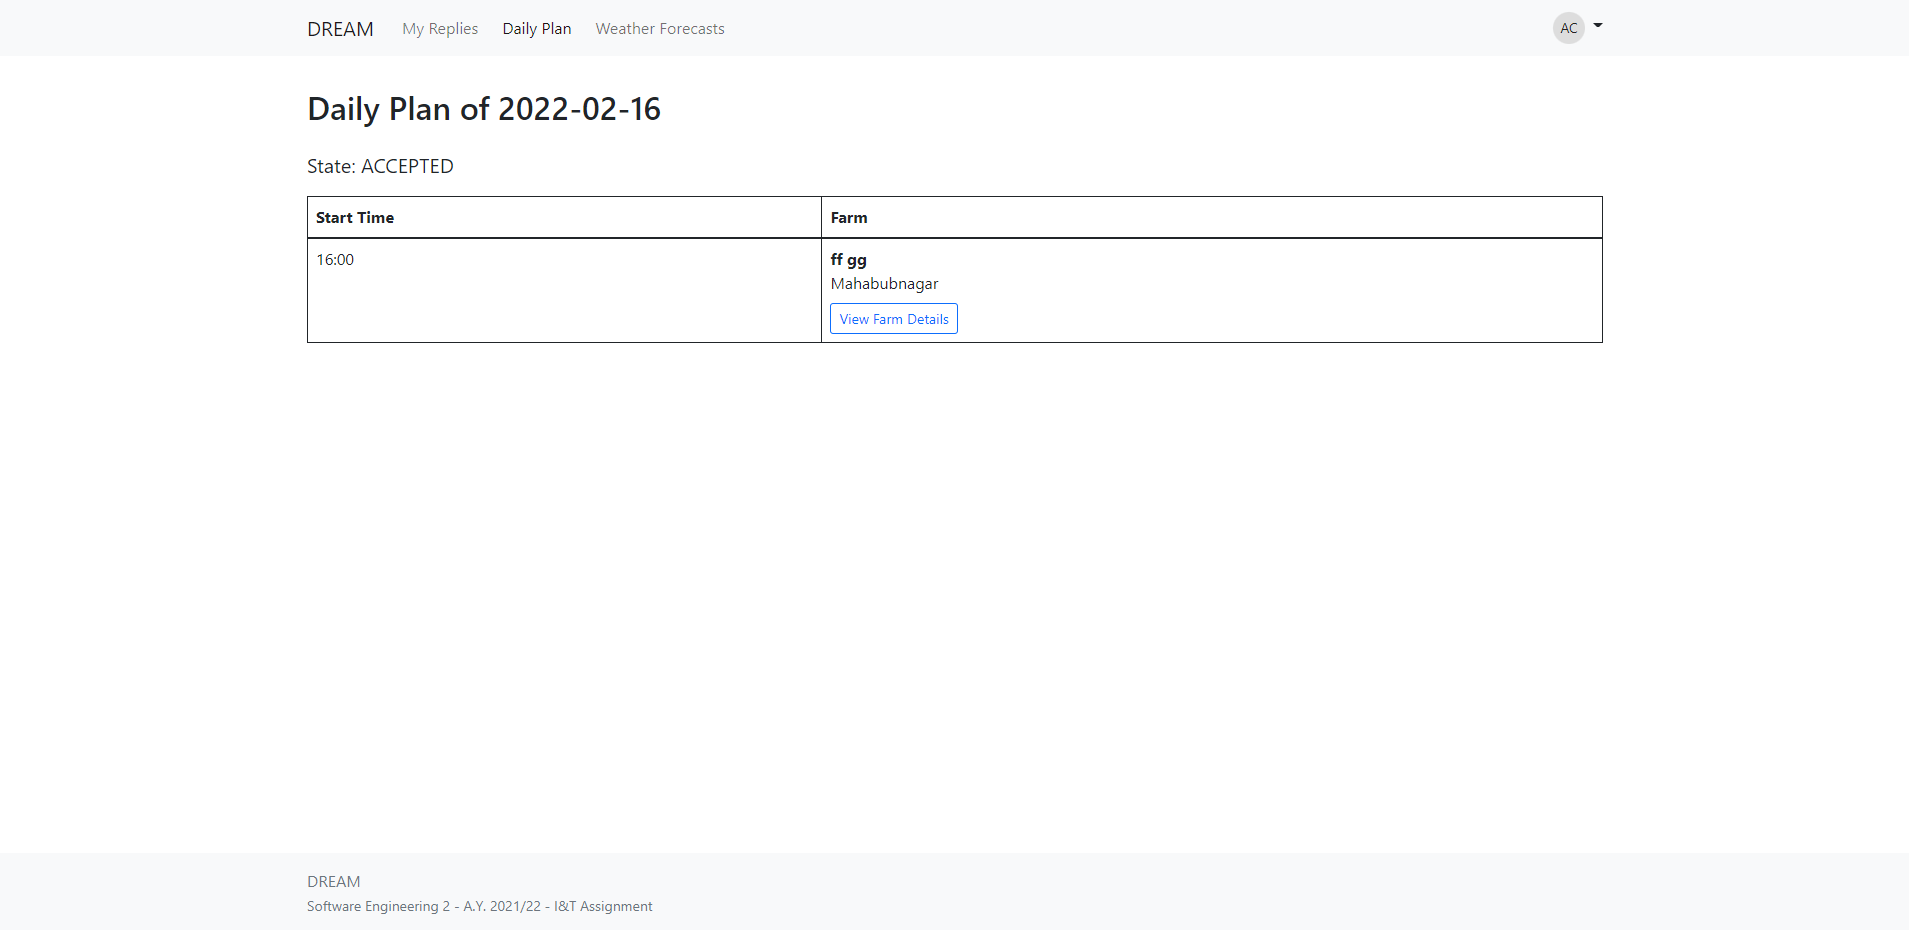
\includegraphics[scale=0.25]{images/additional_notes/view_farm_details.png}
        \caption{Daily Plan section screen}
        \label{fig:my_label}
    \end{figure}
   \newpage
    Error screen:
    \begin{figure}[h!]
        \centering
        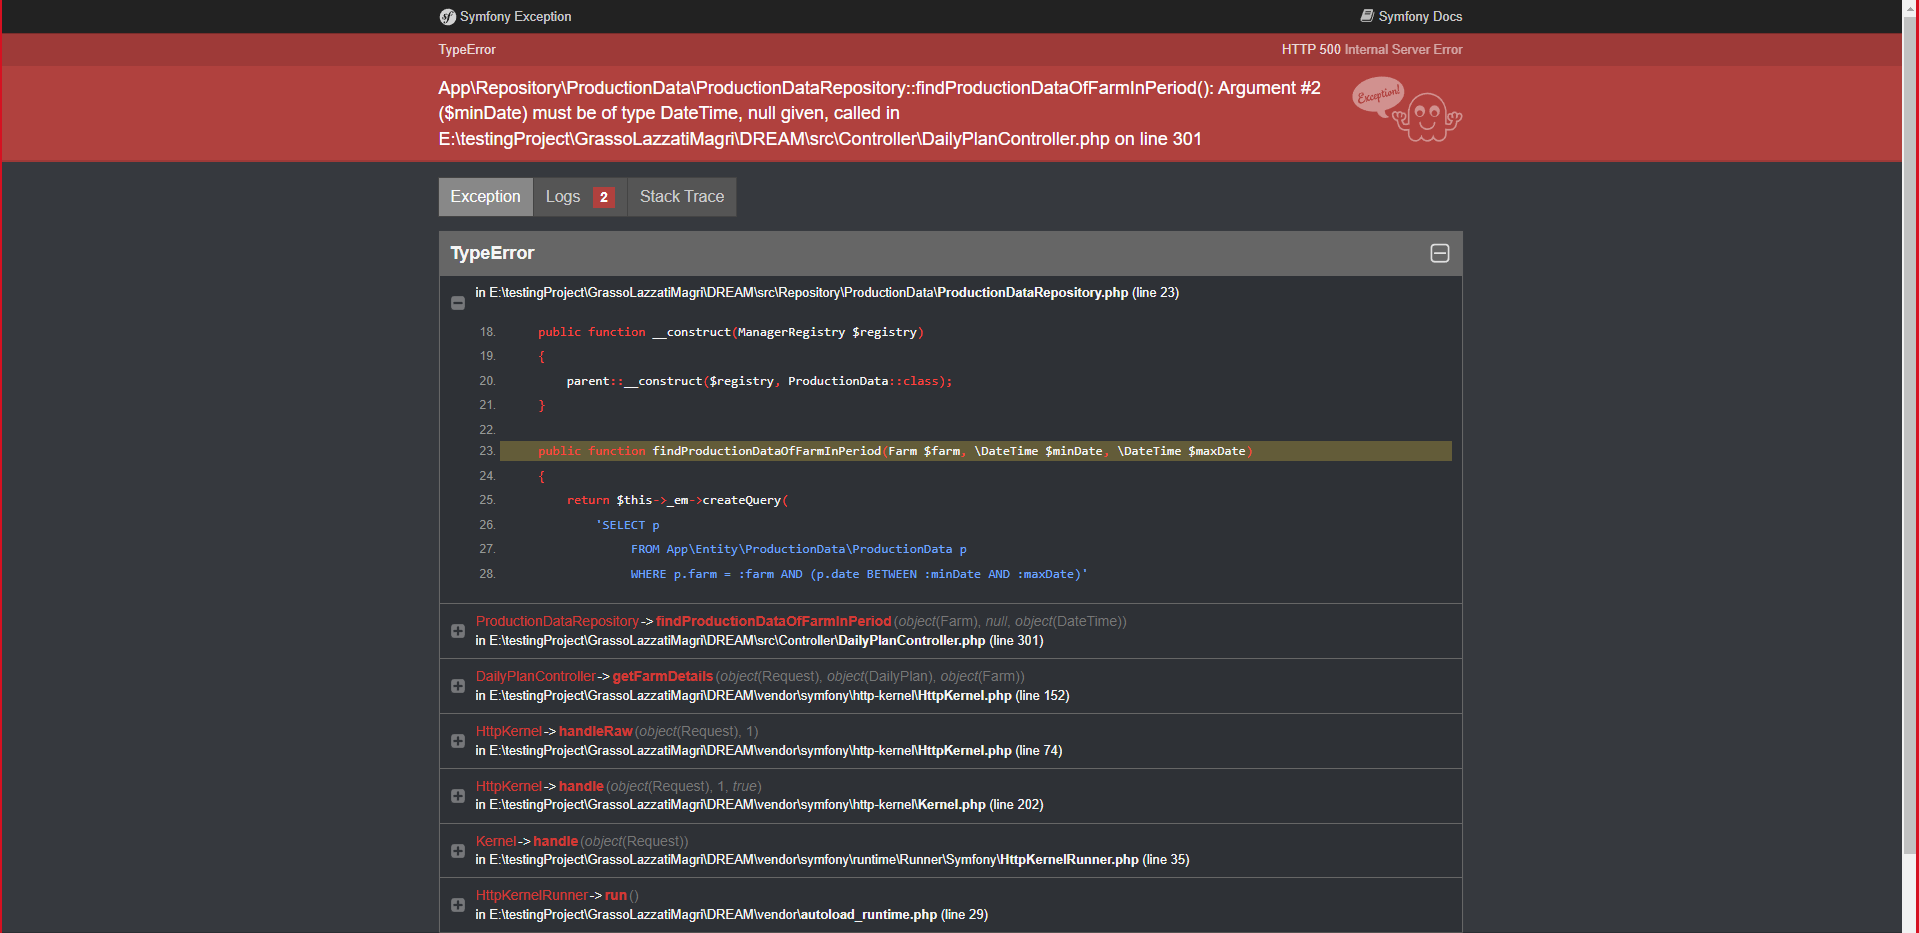
\includegraphics[scale=0.25]{images/additional_notes/view_datail_of_farm_to_visit_agronomist.png}
        \caption{Error retrieved when clicking on View Farm Details}
        \label{fig:my_label}
    \end{figure}
    \FloatBarrier
\end{itemize}


\subsection{User experience concerns}
While testing the application we encountered some terms that were not so clear at first impression.
\begin{itemize}
    \item It's not clear the term "Area" when try to insert a New Production Data. We did not know if we had to indicate an extention or if we had to insert a  maybe the addition of the unit of measure could help understand better.\\
    For instance: Area ($m^2$).
    \item It's not clear the relation between "Farm Area" and "Farm City" for a User. For instance the User, in the registration phase, could select "Adilabad" as Farm Area and "Hyderabad" as Farm City even if "Hyderabad" is the name of another Farm Area.
\end{itemize}